% Springer LNCS report template (draft).
% Compile with: pdflatex report_lncs.tex (twice) OR latexmk -pdf report_lncs.tex
%
% NOTE:
% - This is a PDF-ready draft sized for ~8–12 pages depending on figure placement.
% - Replace author names/IDs and optionally add citations.
\documentclass[runningheads]{llncs}

\usepackage[T1]{fontenc}
\usepackage{graphicx}
\usepackage{booktabs}
\usepackage{listings}
\usepackage{xcolor}
\usepackage{hyperref}
\usepackage{tikz}
\usepackage{pgfplots}
\usepackage{caption}
\usepackage{subcaption}

\hypersetup{
  colorlinks=true,
  linkcolor=blue,
  citecolor=blue,
  urlcolor=blue
}

% ---------- Listings (for JSON/Python snippets) ----------
\definecolor{codebg}{RGB}{248,248,248}
\definecolor{codeframe}{RGB}{220,220,220}
\lstset{
  basicstyle=\ttfamily\small,
  breaklines=true,
  columns=fullflexible,
  frame=single,
  framerule=0.4pt,
  rulecolor=\color{codeframe},
  backgroundcolor=\color{codebg},
  tabsize=2
}

% ---------- TikZ helpers ----------
\usetikzlibrary{arrows.meta, positioning, shapes.geometric, fit}

\begin{document}

\title{AI-Powered Animated Video Generation System:\\From Prompt to Polished Short Film with Modular Agents}

\titlerunning{AI-Powered Animated Video Generation System}

\author{
Umer Farooq\inst{1} \and
Muhammad Usman\inst{2} \and
Muhammad Irtaza Khan\inst{3} \and
Muhammad Ahmed Mufti\inst{4}
}

% Force a short running author header (prevents LNCS from showing
% "Authors Suppressed Due to Excessive Length" in page headers)
\authorrunning{Farooq et al.}

\institute{
National University of Computer and Emerging Sciences (FAST NUCES), Islamabad\\
\email{i220891@nu.edu.pk}
}

\maketitle

\begin{abstract}
We present an end-to-end system that converts a single natural-language prompt into a short animated video with dialogue, character casting, synthesized audio, generated footage, optional lip-sync, and final composition. The system is designed as a modular, phase-oriented pipeline with strict typed contracts enforced using Pydantic. A FastAPI + React web application orchestrates execution, reports real-time status, and enables post-generation edits with versioned undo/redo via file-based state snapshots. We describe the architecture, phase-wise implementation, shared schema, state versioning mechanism, and evaluation-oriented deliverables.
\keywords{Agentic AI \and LLM orchestration \and Text-to-video \and TTS \and State versioning \and Undo/redo}
\end{abstract}

\section{Introduction}
Generating even short animated videos traditionally requires multiple specialist roles and significant production time. Recent progress in generative language, audio, and vision models enables automation, but building a student-accessible pipeline requires careful orchestration, modularity, and robust contracts. This project implements a full-stack system that:
(i) expands a raw user prompt into a structured screenplay, (ii) synthesizes character voices and a timing manifest, (iii) generates per-scene video clips and optionally performs lip-sync, and (iv) composites a final MP4. Finally, an editing interface supports natural-language edit requests and full undo/redo through versioned snapshots.

\section{System Overview}
\subsection{Key Requirements (Project Brief Alignment)}
The system was designed to satisfy the course project phases:
\begin{itemize}
  \item \textbf{Phase 1: Story \& Script} --- prompt $\rightarrow$ structured scenes, dialogue, and character metadata.
  \item \textbf{Phase 2: Audio} --- TTS synthesis and a per-scene timing manifest.
  \item \textbf{Phase 3: Video} --- per-scene generation, A/V synchronization, and export.
  \item \textbf{Phase 4: Web Interface} --- orchestration, progress visibility, preview and download.
  \item \textbf{Phase 5: Edit + Undo} --- interpret edit commands, apply targeted re-generation/recomposition, and maintain version history.
\end{itemize}

\subsection{Architecture Diagram}
Figure~\ref{fig:arch} summarizes the pipeline modules and the shared state contract passed across phases.

\begin{figure}[t]
\centering
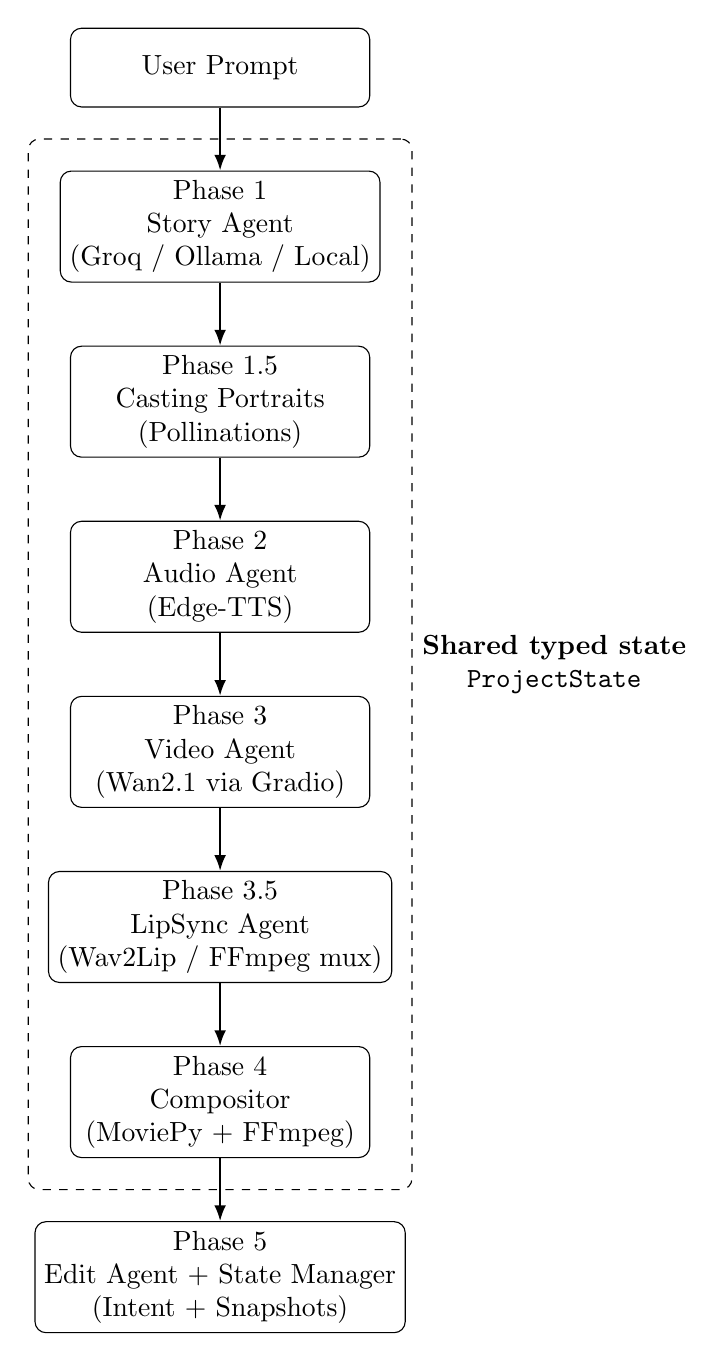
\begin{tikzpicture}[
  node distance=8mm and 10mm,
  box/.style={draw, rounded corners, align=center, minimum width=38mm, minimum height=10mm},
  arrow/.style={-{Latex[length=2.0mm]}, thick}
]
  \node[box] (prompt) {User Prompt};
  \node[box, below=of prompt] (p1) {Phase 1\\Story Agent\\(Groq / Ollama / Local)};
  \node[box, below=of p1] (p15) {Phase 1.5\\Casting Portraits\\(Pollinations)};
  \node[box, below=of p15] (p2) {Phase 2\\Audio Agent\\(Edge-TTS)};
  \node[box, below=of p2] (p3) {Phase 3\\Video Agent\\(Wan2.1 via Gradio)};
  \node[box, below=of p3] (p35) {Phase 3.5\\LipSync Agent\\(Wav2Lip / FFmpeg mux)};
  \node[box, below=of p35] (p4) {Phase 4\\Compositor\\(MoviePy + FFmpeg)};
  \node[box, below=of p4] (p5) {Phase 5\\Edit Agent + State Manager\\(Intent + Snapshots)};

  \draw[arrow] (prompt) -- (p1);
  \draw[arrow] (p1) -- (p15);
  \draw[arrow] (p15) -- (p2);
  \draw[arrow] (p2) -- (p3);
  \draw[arrow] (p3) -- (p35);
  \draw[arrow] (p35) -- (p4);
  \draw[arrow] (p4) -- (p5);

  \node[draw, dashed, rounded corners, fit=(p1)(p4), inner sep=4mm, label={[align=center]right:\textbf{Shared typed state}\\\texttt{ProjectState}}] (statefit) {};
\end{tikzpicture}
\caption{High-level architecture. Each phase consumes/produces a typed \texttt{ProjectState} and assets under \texttt{data/outputs/}.}
\label{fig:arch}
\end{figure}

\section{Shared Data Contracts}
All modules communicate via a single typed state model, minimizing integration ambiguity and enabling snapshotting.

\subsection{Core Models}
We use Pydantic v2 models for strict validation.

\paragraph{Story output.} Scenes contain characters, dialogue, and visual cues for downstream video prompting. Character metadata includes gender and free-text descriptions to support voice and portrait consistency.

\paragraph{Audio timing.} For each scene we store the audio file path, duration, subtitles (optional), and a dialogue timeline with start/end timestamps in seconds. This timeline can drive segment-wise lip-sync.

\paragraph{Project state.} A single \texttt{ProjectState} contains the latest story object, timing manifest, version counter, and an asset map of generated files.

\section{Phase-wise Implementation}
\subsection{Phase 1: Story, Script \& Character Design}
The story module expands a prompt into a structured screenplay. It implements a reliability-first provider cascade:
\begin{itemize}
  \item \textbf{Groq (cloud)} when enabled (fast inference).
  \item \textbf{Ollama (local)} when available for offline runs.
  \item \textbf{Deterministic local fallback} to ensure the pipeline never blocks.
\end{itemize}
The final output is converted into \texttt{StoryOutput} (Pydantic) to prevent unstructured downstream coupling.

\subsection{Phase 1.5: Casting Portraits}
Character portraits are generated using a lightweight web image generation API (Pollinations). The orchestrator extracts unique characters across scenes and generates a portrait per character for UI display and identity anchoring.

\subsection{Phase 2: Audio Generation}
Audio is synthesized using Edge-TTS to produce neural speech without requiring paid keys. For each scene, we generate a final mixed audio file plus a dialogue timeline. The pipeline stores \texttt{audio\_paths} in \texttt{state.assets} and a structured \texttt{TimingManifest} in \texttt{state.timing}.

\subsection{Phase 3: Video Generation}
For each scene, the video agent builds a rich prompt from:
(i) location, (ii) character descriptions, and (iii) dialogue visual cues. Video clips are generated via Wan2.1 served through a Gradio UI, invoked programmatically by a client. If the generator is unreachable, the pipeline falls back to placeholder clips to preserve end-to-end demonstrability.

\subsection{Phase 3.5: Lip-Sync}
The lip-sync agent implements a robust strategy:
\begin{itemize}
  \item If a dialogue timeline exists: split the video into segments by timestamps, apply Wav2Lip (if installed) or FFmpeg mux per segment, and merge.
  \item If no timeline exists: apply whole-scene Wav2Lip or FFmpeg mux fallback.
\end{itemize}
This improves speaker alignment and reduces common failure modes where the first detected face animates across all dialogue.

\subsection{Phase 4: Composition}
The compositor stitches scene clips, aligns audio, and exports \texttt{final\_output.mp4}. Outputs are served via the backend as static files for in-browser preview and download.

\section{Web Orchestration (Phase 4)}
\subsection{Backend (FastAPI)}
The backend provides:
\begin{itemize}
  \item \texttt{POST /api/generate}: start the full pipeline as a background task.
  \item \texttt{GET /api/status/\{job\}}: poll job status/progress and provide portrait paths.
  \item \texttt{POST /api/edit}: apply an edit request to the latest state snapshot.
  \item \texttt{POST /api/undo}, \texttt{POST /api/redo}: state version navigation.
\end{itemize}
Progress is persisted in \texttt{data/temp/<job>.json} to support simple polling and resilience.

\subsection{Frontend (React + Vite)}
The UI provides prompt entry, a phase-aware progress display, cast gallery, a video monitor, and a free-text edit console. Undo/redo buttons call backend endpoints and refresh the video with cache-busting query parameters.

\section{Edit Agent and Versioned Undo (Phase 5)}
\subsection{Intent Parsing and Scoped Execution}
Edit queries are converted into a structured intent object (target, scope, parameters). For the most common use case (scene-specific visual changes), the executor:
\begin{enumerate}
  \item creates an undo snapshot of the current state and assets,
  \item updates the targeted scene prompt,
  \item regenerates only the affected scene clip,
  \item recomposites the final video.
\end{enumerate}

\subsection{State Snapshot Store}
Every run or edit creates a versioned snapshot:
\begin{itemize}
  \item \texttt{data/state\_versions/vX/state.json} --- serialized \texttt{ProjectState}.
  \item \texttt{data/state\_versions/vX/assets/} --- full copy of \texttt{data/outputs/}.
\end{itemize}
Undo/redo restores both the structured state and the physical assets, ensuring reliable replay of previous outputs.

\section{Sequence Diagram (End-to-End Run)}
Figure~\ref{fig:seq} shows the main runtime sequence from a user prompt through the pipeline and snapshot.

\begin{figure}[t]
\centering
\resizebox{\textwidth}{!}{%
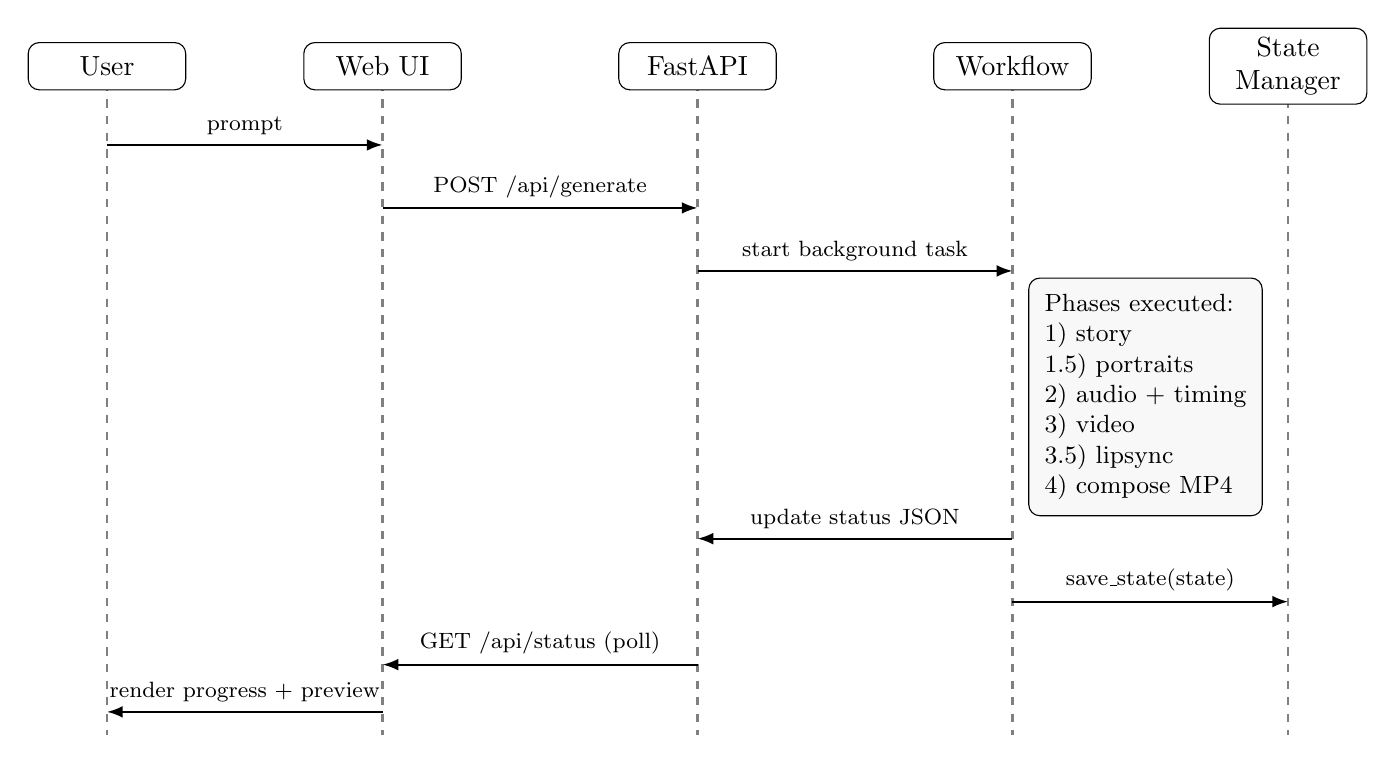
\begin{tikzpicture}[
  lifeline/.style={draw, rounded corners, minimum width=20mm, minimum height=6mm, align=center, fill=white},
  msg/.style={-{Latex[length=2mm]}, thick},
  note/.style={draw, rounded corners, align=left, fill=codebg, inner sep=2mm, font=\small}
]

  % Define X coordinates for vertical lifelines
  \def\uX{0}
  \def\uiX{3.5}
  \def\apiX{7.5}
  \def\wfX{11.5}
  \def\smX{15.0}

  % Draw vertical dashed lifelines
  \draw[dashed, thick, gray] (\uX, 0) -- (\uX, -8.5);
  \draw[dashed, thick, gray] (\uiX, 0) -- (\uiX, -8.5);
  \draw[dashed, thick, gray] (\apiX, 0) -- (\apiX, -8.5);
  \draw[dashed, thick, gray] (\wfX, 0) -- (\wfX, -8.5);
  \draw[dashed, thick, gray] (\smX, 0) -- (\smX, -8.5);

  % Draw actor nodes at the top
  \node[lifeline] (u)   at (\uX, 0) {User};
  \node[lifeline] (ui)  at (\uiX, 0) {Web UI};
  \node[lifeline] (api) at (\apiX, 0) {FastAPI};
  \node[lifeline] (wf)  at (\wfX, 0) {Workflow};
  \node[lifeline] (sm)  at (\smX, 0) {State\\Manager};

  % Forward Messages
  \draw[msg] (\uX, -1) -- node[above, font=\footnotesize]{prompt} (\uiX, -1);
  \draw[msg] (\uiX, -1.8) -- node[above, font=\footnotesize]{POST /api/generate} (\apiX, -1.8);
  \draw[msg] (\apiX, -2.6) -- node[above, font=\footnotesize]{start background task} (\wfX, -2.6);

  % Execution block note attached to the workflow lifeline
  \node[note, anchor=west] (n1) at (\wfX + 0.2, -4.2) {
    Phases executed:\\
    1) story\\
    1.5) portraits\\
    2) audio + timing\\
    3) video\\
    3.5) lipsync\\
    4) compose MP4
  };

  % Return and outgoing messages
  \draw[msg] (\wfX, -6.0) -- node[above, font=\footnotesize]{update status JSON} (\apiX, -6.0);
  \draw[msg] (\wfX, -6.8) -- node[above, font=\footnotesize]{save\_state(state)} (\smX, -6.8);
  \draw[msg] (\apiX, -7.6) -- node[above, font=\footnotesize]{GET /api/status (poll)} (\uiX, -7.6);
  \draw[msg] (\uiX, -8.2) -- node[above, font=\footnotesize]{render progress + preview} (\uX, -8.2);

\end{tikzpicture}%
}
\caption{End-to-end runtime sequence: prompt submission, background orchestration, progress polling, and state snapshotting.}
\label{fig:seq}
\end{figure}

\section{Testing Strategy}
The repository includes phase-level scripts for story, audio, pipeline integration, and edit/undo flows. For grading-oriented completeness, an ideal next step is to convert these into a structured unit test suite (e.g., pytest) and include an intent-classification matrix for at least ten edit query types.

\section{Technology Stack}
\begin{table}[t]
\centering
\caption{Primary technologies used in the implementation.}
\label{tab:stack}
\begin{tabular}{@{}lll@{}}
\toprule
\textbf{Layer} & \textbf{Tech} & \textbf{Purpose} \\
\midrule
Backend & FastAPI + Uvicorn & orchestration endpoints, background tasks \\
Frontend & React + Vite & prompt UI, progress, preview, edit/undo \\
Schemas & Pydantic v2 & strict typed contracts between phases \\
LLM & Groq / Ollama / Local & screenplay generation with fallbacks \\
TTS & Edge-TTS & free neural voice synthesis \\
Portraits & Pollinations API & character casting images \\
Video Gen & Wan2.1 via Gradio client & per-scene footage generation \\
Lip-sync & Wav2Lip + FFmpeg fallback & speaker/scene alignment \\
Composition & MoviePy + FFmpeg & stitch clips and mux audio \\
State Store & file-based snapshots & version history + undo/redo \\
\bottomrule
\end{tabular}
\end{table}

\section{Configuration and Reproducibility}
The system is configured through environment variables loaded from a local \texttt{.env} file. For security, secrets (e.g., API keys) should not be committed; instead, a \texttt{.env.example} can document the expected variables. The configuration used in this implementation is summarized below:
\begin{itemize}
  \item \textbf{LLM providers (Phase 1)}: Groq is optionally supported, but the current configuration uses Ollama locally (\texttt{GROQ\_ENABLED=0}, \texttt{OLLAMA\_ENABLED=1}) with \texttt{OLLAMA\_MODEL=llama3.1:8b} and \texttt{OLLAMA\_BASE\_URL=http://localhost:11434}.
  \item \textbf{Audio (Phase 2)}: Edge-TTS is selected (\texttt{STUDIO\_FLOOR\_VOICE\_BACKEND=edge\_tts}), with rate/pitch controls (\texttt{STUDIO\_FLOOR\_EDGE\_TTS\_RATE}, \texttt{STUDIO\_FLOOR\_EDGE\_TTS\_PITCH}).
  \item \textbf{Video generation (Phase 3)}: the Wan2GP Gradio server is addressed via \texttt{GRADIO\_URL=http://127.0.0.1:42003/}. Some Gradio deployments expose a save-inputs endpoint; this setup uses \texttt{GRADIO\_SAVE\_INPUTS\_API\_NAME=/save\_inputs\_14}.
\end{itemize}

\section{Results and Evidence}
The system produces:
\begin{itemize}
  \item A final composited MP4 at \texttt{data/outputs/final\_output.mp4}.
  \item Versioned snapshots at \texttt{data/state\_versions/v1...vN/}, each containing \texttt{state.json} and full asset copies.
\end{itemize}
These artifacts support demonstration of multi-edit workflows and reliable undo/revert operations.

\section{Limitations and Future Work}
\begin{itemize}
  \item \textbf{Intent parsing}: extending from rule-based parsing to an LLM-based structured classifier (e.g., LangGraph) would better cover diverse edit intents (audio, script, compositing options).
  \item \textbf{Phase-level reruns}: adding explicit endpoints/UI buttons for audio-only regeneration, video-only regeneration, and recompose-only would improve usability and alignment with the brief.
  \item \textbf{Testing}: converting scripts into a CI-ready unit test suite and adding a 10+ intent test matrix would strengthen the Phase 5 deliverable.
\end{itemize}

\appendix
\section{Schema Appendix}
\subsection{StoryOutput (Representative JSON)}
\begin{lstlisting}
{
  "scenes": [
    {
      "scene_id": 1,
      "location": "Rainy Tokyo alleyway",
      "characters": ["Narrator", "Agent K"],
      "character_metadata": {
        "Narrator": { "name": "Narrator", "gender": "male", "description": "calm voice" },
        "Agent K": { "name": "Agent K", "gender": "female", "description": "sharp, observant spy" }
      },
      "dialogue": [
        { "speaker": "Narrator", "line": "The night hides secrets.", "visual_cue": "neon reflections" }
      ]
    }
  ],
  "character_metadata": {
    "Narrator": { "name": "Narrator", "gender": "male", "description": "calm voice" }
  }
}
\end{lstlisting}

\subsection{TimingManifest (Representative JSON)}
\begin{lstlisting}
{
  "scene_timings": {
    "1": {
      "audio_filepath": "data/outputs/audio/scene_01.wav",
      "duration_ms": 8200,
      "subtitle_text": "The night hides secrets.",
      "speaker_tracks": {},
      "dialogue_timeline": [
        { "speaker": "Narrator", "line": "The night hides secrets.", "start_seconds": 0.0, "end_seconds": 3.2 }
      ]
    }
  }
}
\end{lstlisting}

\subsection{ProjectState (Representative JSON)}
\begin{lstlisting}
{
  "version": 5,
  "story": { "...": "StoryOutput" },
  "timing": { "...": "TimingManifest" },
  "assets": {
    "audio_paths": { "1": "data/outputs/audio/scene_01.wav" },
    "video_paths": { "1": "data/outputs/scenes/scene_1.mp4" },
    "synced_video_paths": { "1": "data/outputs/synced/scene_1_synced.mp4" },
    "character_portraits": { "Agent K": "outputs/characters/agent_k.png" }
  }
}
\end{lstlisting}

\section{Environment Variables (Appendix)}
\begin{lstlisting}
# LLM Providers for Story Agent (Phase 1)
GROQ_ENABLED=0
GROQ_API_KEY=
GROQ_MODEL=llama-3.1-8b-instant
GROQ_BASE_URL=https://api.groq.com/openai/v1

OLLAMA_ENABLED=1
OLLAMA_MODEL=llama3.1:8b
OLLAMA_BASE_URL=http://localhost:11434

# Audio (Phase 2)
STUDIO_FLOOR_VOICE_BACKEND=edge_tts
STUDIO_FLOOR_EDGE_TTS_RATE=+0%
STUDIO_FLOOR_EDGE_TTS_PITCH=+0Hz

# Video Generation (Phase 3 - Wan2GP via Pinokio)
GRADIO_URL=http://127.0.0.1:42003/
GRADIO_SAVE_INPUTS_API_NAME=/save_inputs_14
\end{lstlisting}

\end{document}
